\documentclass[a4paper]{article}
\usepackage[spanish]{babel}
\usepackage[utf8]{inputenc}
\usepackage{fancyhdr}
\usepackage{charter}   % tipografia
\usepackage{graphicx}
\usepackage{makeidx}

\usepackage{float}
\usepackage{amsmath, amsthm, amssymb}
\usepackage{amsfonts}
\usepackage{sectsty}
\usepackage{wrapfig}
\usepackage{listings}
\usepackage{caption}

\usepackage{hyperref} %las entradas del índice tienen links
\hypersetup{
    colorlinks=true,
    linktoc=all,
    citecolor=black,
    filecolor=black,
    linkcolor=black,
    urlcolor=black
}

\usepackage{color} % para snipets de codigo coloreados
\usepackage{fancybox}  % para el sbox de los snipets de codigo

\definecolor{litegrey}{gray}{0.94}

% \newenvironment{sidebar}{%
% 	\begin{Sbox}\begin{minipage}{.85\textwidth}}%
% 	{\end{minipage}\end{Sbox}%
% 		\begin{center}\setlength{\fboxsep}{6pt}%
% 		\shadowbox{\TheSbox}\end{center}}
% \newenvironment{warning}{%
% 	\begin{Sbox}\begin{minipage}{.85\textwidth}\sffamily\lite\small\RaggedRight}%
% 	{\end{minipage}\end{Sbox}%
% 		\begin{center}\setlength{\fboxsep}{6pt}%
% 		\colorbox{litegrey}{\TheSbox}\end{center}}

\newenvironment{codesnippet}{%
	\begin{Sbox}\begin{minipage}{\textwidth}\sffamily\small}%
	{\end{minipage}\end{Sbox}%
		\begin{center}%
		\colorbox{litegrey}{\TheSbox}\end{center}}



\usepackage{fancyhdr}
\pagestyle{fancy}

%\renewcommand{\chaptermark}[1]{\markboth{#1}{}}
\renewcommand{\sectionmark}[1]{\markright{\thesection\ - #1}}

\fancyhf{}

\fancyhead[LO]{Sección \rightmark} % \thesection\
\fancyfoot[LO]{\small{Martín Caravario, Federico Hosen, Lucas Vuotto}}
\fancyfoot[RO]{\thepage}
\renewcommand{\headrulewidth}{0.5pt}
\renewcommand{\footrulewidth}{0.5pt}
\setlength{\hoffset}{-0.8in}
\setlength{\textwidth}{16cm}
%\setlength{\hoffset}{-1.1cm}
%\setlength{\textwidth}{16cm}
\setlength{\headsep}{0.5cm}
\setlength{\textheight}{25cm}
\setlength{\voffset}{-0.7in}
\setlength{\headwidth}{\textwidth}
\setlength{\headheight}{13.1pt}

\renewcommand{\baselinestretch}{1.1}  % line spacing


\usepackage{underscore}
\usepackage{caratula}
\usepackage{url}

\usepackage{color}
\usepackage{clrscode3e} % para el pseudocodigo




\begin{document}

\lstset{
  language=C++,
  backgroundcolor=\color{white},   % choose the background color
  basicstyle=\footnotesize,        % size of fonts used for the code
  breaklines=true,                 % automatic line breaking only at whitespace
  captionpos=b,                    % sets the caption-position to bottom
  commentstyle=\color{mygreen},    % comment style
  escapeinside={\%*}{*)},          % if you want to add LaTeX within your code
  keywordstyle=\color{blue},       % keyword style
  stringstyle=\color{mymauve},     % string literal style
}

\thispagestyle{empty}
\materia{Sistemas Operativos}
\submateria{Segundo Cuatrimestre de 2014}
\titulo{Trabajo Práctico II}
%\subtitulo{}
\integrante{Caravario, Martín}{470/12}{martin.caravario@gmail.com}
\integrante{Hosen, Federico}{825/12}{fhosen@hotmail.com}
\integrante{Vuotto, Lucas}{385/12}{lvuotto@dc.uba.ar}

\maketitle
\newpage

\thispagestyle{empty}
\vfill
\begin{abstract}
    \vspace{0.5cm}
    \textcolor{red}{\textbf{completar!}}
\end{abstract}

\thispagestyle{empty}
\vspace{1.5cm}
\tableofcontents
\newpage


%\normalsize
\newpage
\tableofcontents

\section{Objetivos generales}
\textcolor{red}{\textbf{completar!}}

\newpage

\section{Plataforma de pruebas}

\textcolor{red}{\textbf{chequear!}} \medskip

El testeo de los algoritmos implementados fue realizado, principalmente, en las máquinas del laboratorio 3 del DC. \newline
\begin{itemize}
  \item \textbf{Sistema Operativo:} Ubuntu Linux 12.04 x86_64, kernel 3.2.0-30-generic

  \item \textbf{Especificaciones del Software:} el código está implementado en \textbf{C++}, compilado con \verb|-std=c++0x|.
  Utilizamos \textbf{Bash} y \textbf{Ruby} para los scripts. Los gráficos fueron realizados con \textbf{gnuplot}.

  \item \textbf{Especificaciones del Hardware:} Intel(R) Core(TM) i5-2500K CPU @ 3.30GHz, 8GB de RAM.
\end{itemize}

\newpage


 \section{Ejercicio 1}

 \subsection{Explicacion del algoritmo}
 Para este ejercicio lo que hicimos fue crear una funci\'on llamada
 \textbf{get\_rand} a la cual le pasamos los parametros bmin y bmax. El
 objetivo de esta funcion era generar un numero aleatorio entre bmin y bmax,
 lo cual logramos de la siguiente manera:
 \begin{verbatim}

 return rand() % (bmax - bmin + 1) + bmin;

 \end{verbatim}

 Cabe destacar que utilizamos la funcion rand(), la cual fue sugerida por la
 catedra, con el fin de generar un numero aleatorio.
 Esta funci\'on es invocada n veces, siendo n el numero de veces que la
 tarea debe ser bloqueada, dentro del ciclo principal de la tarea, con el
 fin de generar n numeros aleatorios diferentes que seran utilizados como la
 duracion de cada llamada bloqueante.




\textbf{\textcolor{red}{¡COMPLETAR CON EL INFORME!}}

\section{Ejercicio 3: Round Robin}

\subsection{Explicación del algoritmo.}
El tipo de scheduling \textit{round robin} consiste en asignar a cada proceso un
tiempo predeterminado para que ejecute, llamado \textit{quantum}. Si el proceso no termina su ejecución antes de que se
acabe su ración de tiempo, es desalojado y puesto en una cola (espera
circular) para ser retomada su ejecución luego de atender a los demás
procesos en dicha cola.

Este modelo de scheduling permite asegurarse de que no exista
\textit{starvation}, pues todos los procesos son atendidos; y no sólo eso,
si no que a todos lo procesos les es asignado el mismo quantum. De esta
forma, round robin es altamente confiable en términos de \textit{fairness}.

Para implementarlo utilizamos una cola \footnote{Implementada con
\textit{queue} de la STL de C++.}, de nombre
\textit{ready} que nos indica las tareas en espera para su ejecución.
Utilizamos también dos vectores \footnote{Implementados con
\textit{vector} de la STL de C++.} de enteros, \textit{ticks} y
\textit{quantums}. En el primero guardamos la cantidad de ciclos restantes
para la tarea que está corriendo en cada núcleo, y en el segundo tenemos
almacenados los quantums correspondientes a cada núcleo. 

Dado un núcleo, cuando el elemento de \textit{ticks} correspondiente a dicho
núcleo alcanza el valor \textit{0}, dicho proceso es desalojado y puesto en
el final de la cola, dejando el procesador libre para el próximo en la cola.
Si no existe algún proceso en la cola, la \textit{idle} es puesta a correr.

De igual forma, cuando un proceso se bloquea, es puesto de vuelta en la
cola, y la próxima vez que corra lo hará con el \textit{quantum} entero.
Ésto es, quizás, una de las falencias de esta implementación \textit{naive}
de \textit{round robin}, en términos de \textit{fairness}, pues la tarea que
se bloquea \textit{pierde} una porción de su tiempo asignado, que no es
recuperado en su siguiente turno. Una posible modificación a la
implementación para solucionar esto sería añadir algún sistema de
recompensas para las tareas que no terminan su \textit{quantum}.

\section{Ejercicio 4: Simulaciones y análisis de Round Robin}

\subsection{Introducción}
En este ejercicio vamos a analizar el comportamiento del modelo de
scheduling \textit{Round Robin} variando la cantidad de tareas, el quantum,
la cantidad de núcleos, y el tiempo de cambio de contexto.
La idea es ver como éstas variaciones afectan las distintas métricas
mencionadas anteriormente, para así llegar a alguna conclusión sobre este
scheduler.

\subsection{Experimento 1: Funcionamiento RR}
En este primer experimento vamos a simular 8 tareas de uso intensivo de CPU
con un procesador de un núcleo, fijando el costo de cambio de contexto en 1,
con un quantum fijo, y con \textit{release time} pseudoaleatorio.

El objetivo de este experimento es verificar que el round robin se comporte
de la manera esperada, es decir, la mencionada en el ejercicio 3.

Primero simularemos un lote de 8 tareas de uso intensivo del cpu, con un
costo de cambio de contexto de 1, en un procesador de 1 núcleo. Luego
simularemos en el mismo entorno, pero con un lote de 8 tareas varias (uso
intensivo y  taskConsola).

El lote de tareas utilizado fue el siguiente:

\begin{verbatim}
TaskCPU 15
TaskCPU 11
TaskCPU 25
TaskCPU 24
TaskCPU 10
TaskCPU 16
TaskCPU 13
TaskCPU 22
\end{verbatim}

\subsubsection{Resultados}
\begin{figure}[htb]
\begin{center}
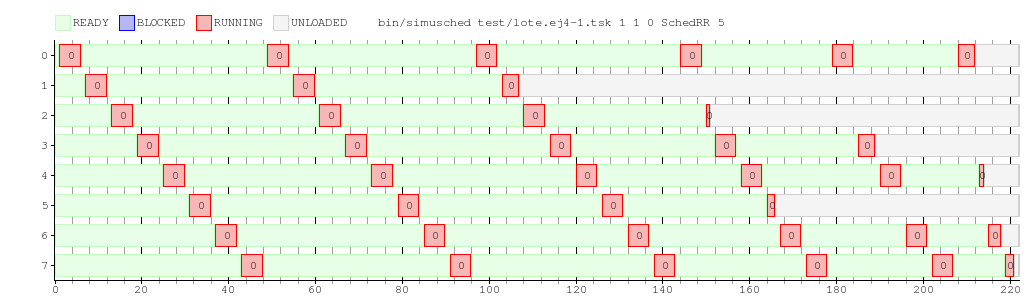
\includegraphics[scale=0.4]{imagenes/ej4-1.png}
\end{center}
\caption{Experimento 1. Lote 8 tareas. Quantum 5.}
\end{figure}

\subsubsection{Conclusión}
Como era de esperarse, empieza a ejecutarse el primer proceso \textit{listo}
hasta cumplir su cuota de tiempo, luego pasa a ejecutar al siguiente, y así
hasta retomar la primer tarea (pues se turnan de manera circular). A medida
que los procesos terminan la totalidad de su ejecución, la cola se va haciendo más corta,
acortando el tiempo de espera entre el desalojo de un proceso y su retorno.
Ésto se repite hasta que todos los procesos terminan su ejecución.

\subsection{Experimento 2: Impacto del quantum}
La idea de este experimento es analizar el impacto del tamaño del quantum en el turnaround. Tener un quantum muy bajo haría que dicha métrica se reduzca,
dado que habrá mas ciclos de reloj dedicados a realizar los cambios de
contextos, aumentando el tiempo total que le tomas a las tareas terminar su
ejecución. Pero si ésta es demasiado alta podría generar que el tiempo de
respuesta percibido sea muy alto, pero como no nos interesa medir esta
métrica, no lo tendremos en cuenta.

Analizaremos primero comparativamente en un procesador de un núcleo, con el
mismo lote de tareas, variando el quantum.

Procesador de 1 núcleo, con un quantum de valor 2.

Procesador de 1 núcleo, con un quantum de valor 7.

Procesador de 1 núcleo, con un quantum de valor 15.

Ahora analizamos comparativamente en un procesador de 4 núcleos, manteniendo
el mismo lote de tareas, y tomando los mismo valores de quantum (en 3
simulaciones distintas).

Procesador de 4 núcleos, con un quantum de valor 2.

Procesador de 4 núcleos, con un quantum de valor 7.

Procesador de 4 núcleos, con un quantum de valor 15.

\subsubsection{Conclusión}

\subsection{Ejercicio 5: Lottery Scheduling}
\subsubsection{Explicación del algoritmo}
El modelo de scheduling \textit{Lottery} consiste en tener un sistema
pseudoaleatorio que decida cual va a ser el siguiente proceso a ser
ejecutado. Esto lo hace \textit{repartiendo tickets} a cada proceso, y
generando un ticket ganador al azar. Así, cada
proceso va a tener asociado una cantidad de tickets, obteniendo
cierta probabilidad de ganar la lotería. De esta forma, el proceso con más
tickets tiene más probabilidades de ganar. Éste es el mecanismo que nos
permite establecer relaciones de prioridades entre procesos.
Y como dado un número entre $1$ y $n$, la posibilidad de que dicho número
\textbf{no} salga nunca es $0$, eventualmente el número será elegido por el
algoritmo de scheduling. De esta forma, no hay \textit{starvation}, pues
todo proceso será puesto a correr en algún momento.

Para implementarlo utilizamos:
\begin{itemize}
\item Una lista de procesos y sus tickets, \textbf{procesos}
\footnote{Utilizamos \verb|list<pair<int,int> >| de la STL de C++.}.
\item Un diccionario de procesos bloqueados, \textbf{bloqueados}
%\footnote{Utilizamos \verb|map<int,int>| de la STL de C++. }, que dado un pid guarda con cuantos
%tickets tiene que regresar.
\item Una variable entera \textbf{ciclos}, que especifica cuantos ciclos
consumió el proceso actual (el que ocupa el procesador).
\item Una variable entera \textbf{quantum}.
\item Una variable entera \textbf{tickets}, que indica la cantidad de
tickets totales asignados.
\end{itemize}

\newpage

\section{Apéndice 1: acerca de los tests}

\textcolor{red}{\textbf{chequear!}} \medskip

Los \textbf{casos aleatorios se generan mediante los scripts} (en Ruby) \verb|ejN.random.rb|, donde
N es el número correspondiente al problema. Estos scripts toman siempre \textbf{dos parámetros},
siendo el primero la semilla que utilizamos para generar números pseudoaleatorios, que
\textbf{por defecto toma el valor 0} si no es especificado y \textbf{el segundo parámetro corresponde
al tamaño de la entrada}.

Además de los tests con casos aleatorios, \textbf{tenemos en cuenta los mejores y peores
casos de cada algoritmo}, fijando los valores adecuados de los parámetros para
obtenerlos. \medskip

En cuanto a la metodología para medir el tiempo, utilizamos el archivo \verb|tiempo.h|,
que define macros para contar la \textbf{cantidad de ciclos de clock} producidos entre dos instantes. \medskip

Cada instancia se repite varias veces para reducir el impacto de los \textit{outliers}, quedándonos
con el \textbf{valor mínimo} en cada caso. Estos valores (de entrada y salida) se vuelcan a un archivo
\verb|info.n.dat| dentro de la carpeta \textit{benchmark}, que es utilizado luego para generar los gráficos
mediante \textbf{gnuplot}. \medskip

Para correr los tests estáticos (sin variables aleatorias), se ejecuta \verb|make; make test| y para los
casos aleatorios (utilizados para los gráficos), \verb|make; make plot|.

Todos los archivos \verb|.cc| son compilados utilizando la optimización \verb|-O3|. \medskip

Tener en cuenta que, a pesar de ejecutar los tests reiteradas veces, aún es posible que estén presentes ciertos
valores atípicos (menores o mayores a los esperados), ya sea por optimizaciones que realice el procesador, sobrecarga
del mismo, etc.
\newpage

\section{Apéndice 2: secciones relevantes del código}

\textcolor{red}{\textbf{chequear!}} \medskip

En esta sección, adjuntamos parte del código correspondiente a la resolución de cada problema
que consideramos más \textbf{relevante}. Omitimos los encabezados, bibliotecas incluídas,
funciones \verb|main| y de impresión de resultados. El código se encuentra comentado en los
archivos \verb|.cc|.

\subsection{Código del Problema 1}


\begin{lstlisting}
\end{lstlisting}

\vspace*{0.5cm}


\newpage


\subsection{Código del Problema 2}


\begin{lstlisting}
\end{lstlisting}

\vspace*{0.5cm}


\newpage


\subsection{Código del Problema 3}


\begin{lstlisting}
\end{lstlisting}

\vspace*{0.5cm}


\end{document}
